% This is samplepaper.tex, a sample chapter demonstrating the
% LLNCS macro package for Springer Computer Science proceedings;
% Version 2.20 of 2017/10/04
%
\documentclass[runningheads]{llncs}
%
\usepackage{graphicx}
\graphicspath{ {./img/} }
\usepackage{listings}
\usepackage{xcolor}

\colorlet{punct}{red!60!black}
\definecolor{background}{HTML}{EEEEEE}
\definecolor{delim}{RGB}{20,105,176}
\colorlet{numb}{magenta!60!black}

\newcommand\blfootnote[1]{%
\begingroup
\renewcommand\thefootnote{}\footnote{#1}%
\addtocounter{footnote}{-1}%
\endgroup
}

\lstdefinelanguage{json}{
    basicstyle=\normalfont\ttfamily,
    stepnumber=1,
    numbersep=8pt,
    showstringspaces=false,
    breaklines=true,
    frame=lines,
    backgroundcolor=\color{background},
    literate=
     *{0}{{{\color{numb}0}}}{1}
      {1}{{{\color{numb}1}}}{1}
      {2}{{{\color{numb}2}}}{1}
      {3}{{{\color{numb}3}}}{1}
      {4}{{{\color{numb}4}}}{1}
      {5}{{{\color{numb}5}}}{1}
      {6}{{{\color{numb}6}}}{1}
      {7}{{{\color{numb}7}}}{1}
      {8}{{{\color{numb}8}}}{1}
      {9}{{{\color{numb}9}}}{1}
      {:}{{{\color{punct}{:}}}}{1}
      {,}{{{\color{punct}{,}}}}{1}
      {\{}{{{\color{delim}{\{}}}}{1}
      {\}}{{{\color{delim}{\}}}}}{1}
      {[}{{{\color{delim}{[}}}}{1}
      {]}{{{\color{delim}{]}}}}{1},
}

% Used for displaying a sample figure. If possible, figure files should
% be included in EPS format.
%
% If you use the hyperref package, please uncomment the following line
% to display URLs in blue roman font according to Springer's eBook style:
% \renewcommand\UrlFont{\color{blue}\rmfamily}

\begin{document}
%
\title{Third-party Payment Specification for MaaS}
%
%\titlerunning{Abbreviated paper title}
% If the paper title is too long for the running head, you can set
% an abbreviated paper title here
%
\author{Brecht Van de Vyvere\inst{1}\orcidID{0000-0002-7671-6203} \and
Tim Asperges\inst{2} \and \\
Pieter Colpaert\inst{1}\orcidID{0000-0001-6917-2167} \and \\
Ruben Verborgh\inst{1}\orcidID{0000-0002-8596-222X}}
%
\authorrunning{B. Van de Vyvere et al.}
% First names are abbreviated in the running head.
% If there are more than two authors, 'et al.' is used.
%
\institute{IDLab, Department of Electronics and Information Systems,\\ Ghent University – imec
\email{\{brecht.vandevyvere,pieter.colpaert,ruben.verborgh\}@ugent.be}\\
\url{https://idlab.technology/} \and
City of Leuven, Belgium\\
\email{tim.asperges@leuven.be}}
%


\maketitle              % typeset the header of the contribution
%
\begin{abstract}
Mobility as a service (MaaS) allows intelligent transportation across multiple mobility providers, such as calculating the least expensive route. However, the current standards do not tackle third-party payments (TPPs) where a third party compensates a part of a travellers’ trip cost when certain criteria are met. For example, travellers receive 10\% discount from a local government when renting a shared bike in the cities' centre during peak hours. To automatize TPP agreements for MaaS, we propose and demonstrate with an example (i) a specification to set up a TPP system specifying, among others, how multimodal criteria and trips can be semantically described, and (ii) an open source validator tool returning the compensation for a trip. In future work, we are investigating how personal data can be integrated using Solid data pods.

\keywords{Third-party payments \and Mobility as a Service \and Local decisions.}
\end{abstract}
%
%
%
\section{Introduction}

\blfootnote{Copyright \textsuperscript{\textcopyright} 2021 for this paper by its authors. Use
permitted under Creative Commons License Attribution 4.0 International (CC BY 4.0).}

Standardized data models (General Transit Feed Specification (GTFS) \cite{gtfs}, Mobility Data Specification (MDS) \cite{mds}) or Web Application Programming Interfaces (APIs) (General Bikeshare Feed Specification (GBFS) \cite{gbfs}, Transport Operator, MaaS Provider (TOMP) API \cite{tompapi}) allow MaaS providers to calculate the financial cost of a trip for transportation. However, this does not exist for third-party payment schemes. The term 'third-party payment' (TPP) in the context of MaaS refers to the compensation a traveller receives from a third party, such as a local government, when a trip is performed compliant with the third parties' criteria, such as student discounts. Next to the regular payment from the traveller to the used mobility service, a second payment is performed from the third party to the traveller or service, depending on the implementation of the TPP system (see Section \ref{section:tpp}). According to the overview provided in Table \ref{table-tpp}, some TPP systems are already set up between local governments and mobility providers to increase the accessibility of shared mobility to certain groups, such as tourists or children, or during an event. These criteria are based on location, time, transport modality and traveller's profile information and are defined in local decisions in the form of subsidy measurements. A TPP system can be achieved in a pre- or postpaid fashion. From the view point of a traveller, with prepaid, a smaller part of the trip must be paid by the traveller: a \emph{split bill} occurs where the second part is arranged between the third party and mobility provider. With postpaid, a traveller pays the total trip cost to the mobility provider and receives its compensation afterwards from the third party. Based on the advice of some cities (Leuven, Antwerp), we will focus in this article on prepaid so groups with a low income or certain social background can be compensated on the moment of ticketing. Prepaid can be implemented with vouchers or mobility budget containing, for example, free rides or credit. Another approach is an agreement describing the subsidy measurement criteria and how a mobility provider can send an invoice afterwards to the third party. Currently, these TPPs are made ad hoc lowering the discoverability and reusability for route planning advice in MaaS. Therefore, we propose a specification for a prepaid TPP system defining the semantic description of subsidy measurements and trips, and an open-source validator to verify whether a trip is compliant with a subsidy measurement.

\begin{table}
\caption{State of play of third-party payment schemes in Flanders.}\label{tab1}
\begin{tabular}{| p{0.10\linewidth} | p{0.34\linewidth} | p{0.14\linewidth} | p{0.34\linewidth}|}
\hline
City &  Description & Provider & Criteria\\
\hline
Deinze &  Free rides with shared bikes & Blue Bike & Location of the trip must be in Deinze\\
Leuven & Free rides with bus & De Lijn & Citizens younger than 12 years of district Leuven\\
Leuven & Discount on public transport & NMBS and De Lijn & During certain events\\
Schoten & Vouchers for 20 minutes free rides with shared bike & Mobit & During certain events \\
\hline
\end{tabular}
\label{table-tpp}
\end{table}

\section{Third-party payment specification for MaaS}
\label{section:tpp}

\subsection{Preliminaries}

Open Standards for Linking Organizations (OSLO) \cite{buyle_egose_2016}, a program of the Flanders Information Agency enables organizations in Flanders to cooperate in trajectories, to develop unambiguous standards for information exchange. The “OSLO mobility: trips and offer” standard \cite{tripsandoffer} was triggered by the new decree Basic Accessibility in Flanders \cite{ba}, which states that important social locations must be optimally accessible to travellers. To realize this, a traveller must have a clear view on the existing mobility offer and on how to interconnect the various transport options in a multimodal mobility context. The standard consists of a vocabulary for describing trips, transport networks and service offerings, and of a “trips and offer” application profile (AP). The AP specifies which data needs to be exchanged concerning i) trips done by users and ii) the mobility services at their disposal. This AP allows mobility providers to describe trips in a machine-readable way.

The Local Council Decisions as Linked Open Data (LBLOD) programme is a Flemish initiative to semantically annotate decisions of local governments \cite{buyle_iswc_demo_2016}. Local administrations currently have to upload  decisions from their organization into Flemish base registries, such as the database for mandates, or road signs. By embedding RDFa in their documents, the Flemish government and third parties can harvest the information  themselves in an automatic way, similarly to search engines that harvest Schema.org annotations from websites. LBLOD has already initiated several OSLO trajectories for domain-specific decisions, such as the installment or removal of mandataries \cite{mandate}, traffic \cite{trafficmeasurement} and subsidy regulations \cite{subsidymeasurement}. The “subsidies” AP reuses terms from the European ISA standard Core Criterion and Core Evidence Vocabulary (CCCEV) \cite{cccev} to describe criteria, requirements and how to group them. This AP allows local governments to define  TPP subsidy measurements, its criteria and monetary compensation in a machine-readable way.

\subsection{System overview}

The TPP specification describes the steps local governments and mobility operators can perform to compensate a travellers' trip \cite{tpp}. According to the overview provided in Fig. \ref{fig:tppdiagram}, the system starts with the local government (agency), that defines which trips can be compensated (i). When a MaaS provider can implement the subsidy and conforms with the cities' quality framework (QF), a TPP agreement can be arranged (ii), which is annotated according to the LBLOD AP for subsidies \cite{subsidymeasurement}. The trip of a user is described with the OSLO AP “trips and offer” \cite{tripsandoffer} (iii) and can be validated with the semantically annotated agreement (iv). When a trip meets the criteria, the validator returns how much can be compensated (v). For reimbursement, the mobility provider sends an invoice with the number of trip compensations (vi). In future work, the agency should be able to verify with the validator whether the compensated trips in the report are legitimate. To do so, the report will also need to embed the machine-readable description of the compensated trips as proof.

\begin{figure}
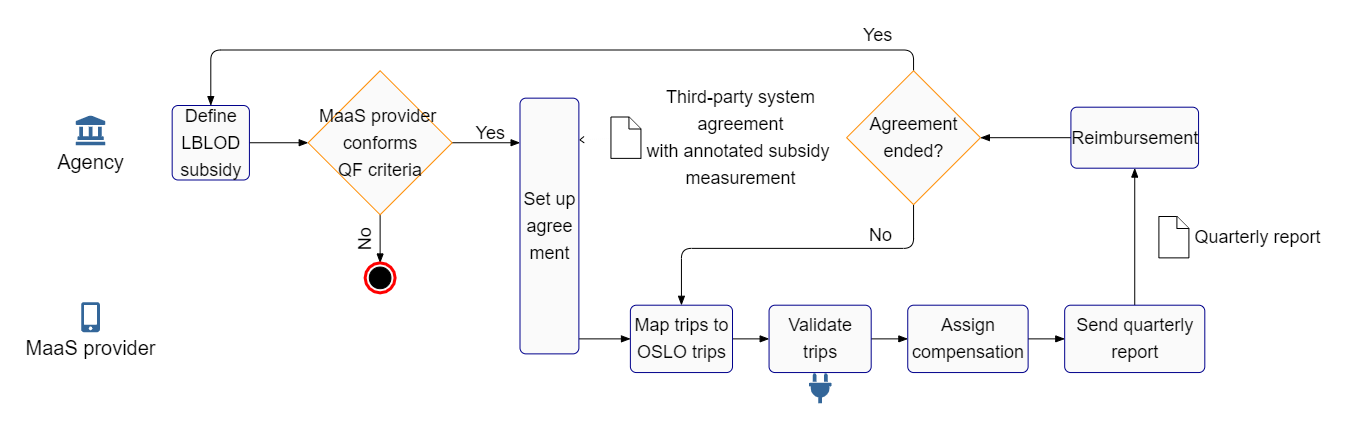
\includegraphics[width=\textwidth]{tppdiagram.png}
\caption{Overview of setting up a TPP scheme between an agency (top row) and MaaS provider (bottom row).} 
\label{fig:tppdiagram}
\end{figure}


\subsection{Example}

Inspired by projects like MDS \cite{mds} and LBLOD \cite{subsidymeasurement}, we specify which standards to use to describe subsidy measurements and trips, and how trips can be validated in an automated fashion. We provide a JavaScript Object Notation Linked Data (JSON-LD) template with corresponding table for each type of object. 
This way, developers do not need to understand semantic technologies to start mapping their data. A JSON-LD context is added to make the template semantically interoperable. 
In Listing \ref{list:requirement}, we give an example of a requirement for shared bikes in Leuven. Next to \emph{RouteSegmentRequirements}, an  agency also needs to describe the \emph{SubsidyMeasurement}, which combines multiple requirements, and \emph{Payment} indicating how much will be compensated. More details can be found on the Github repository of the specification\cite{tpp}. 

Similarly, providers need to map every trip to "trips and offer"\cite{tripsandoffer}. A trip executes a certain route composing multiple route segments. These segments specify the departure and arrival time, GPS telemetry, price and transport modality. For example, Listing  \ref{list:routesegment} demonstrates a shared bike system during rush hours costing 8.2 Euro. 

With the standardized description of a trip and subsidy measurement as input, an open source validator is being developed returning whether a trip is conform with the subsidy measurement and how much compensation can be given \cite{tpp}. MaaS providers can incorporate this tool into their route planning engine. Also, agencies could use this tool as validation step before payment.

\begin{lstlisting}[language=json, caption={Travellers are eligible for a subsidy measurement when they use a shared bicycle within the centre of Leuven and on a monday during rush hours.}, label={list:requirement}
]
{ "@type": "RouteSegmentRequirement",
  "description": "Only shared bikes, on monday between 4pm and 6pm and used in the city centre of Leuven.",
  "meansOfTransport": "http://www.wikidata.org/entity/Q1358919", // Bike
  "location": {
  	"@type": "Place",
    "geometry": {
      "wkt": "POLYGON((4.676055908203124 50.88993205766312...))" }
  },
  "time": [{
    "@type": "OpeningHoursSpecification",
    "dayOfWeek": "http://schema.org/Monday",
    "startTime": "15:00:00"
    "endTime": "18:00:00"
  }]
}
\end{lstlisting}

\begin{lstlisting}[language=json, caption={This route segment is performed during rush hours in the centre of Leuven with a shared bike system.}, label={list:routesegment}]
{
  "@type": "RouteSegment",
  "departureTime": "2020-06-09T16:01:00",
  "arrivalTime": "2020-06-09T17:05:00",
  "telemetry": [ "..." ],
  "price": {
     "@type": "MonetaryAmount",
     "value": "8.2",
     "currency": "EUR"
 },
  "meansOfTransport": "http://www.wikidata.org/entity/Q1358919" // Shared bike
}
\end{lstlisting}

\section{Conclusion}

The specification and validator proposed in this demo set the first steps towards third-party payments for MaaS. In future work, we want to make TPPs on the one hand more inclusive and on the other hand use the validator in a generic, cross-domain incentives (subsidy measurements) platform. Both aspects require the use or creation of personal data: the validator will need to be extended to handle profile information, and incentives should be assignable to a person. As cities nor MaaS operators should be responsible for managing personal data, we are looking into using Solid data pods, an innovative data storage solution for private data. With this last element added, we hope to have an interesting discussion during the workshop about the future ecosystem of TPPs for MaaS.

%
% ---- Bibliography ----
%
% BibTeX users should specify bibliography style 'splncs04'.
% References will then be sorted and formatted in the correct style.
%
\bibliographystyle{splncs04}
\bibliography{mybibliography}
%

\end{document}
